\documentclass[10pt,twocolumn,letterpaper]{article}

\usepackage{cvpr}
\usepackage{times}
\usepackage{epsfig}
\usepackage{graphicx}
\usepackage{amsmath}
\usepackage{amssymb}
\usepackage{float}

% Include other packages here, before hyperref.

% If you comment hyperref and then uncomment it, you should delete
% egpaper.aux before re-running latex.  (Or just hit 'q' on the first latex
% run, let it finish, and you should be clear).
\usepackage[breaklinks=true,bookmarks=false]{hyperref}

\cvprfinalcopy % *** Uncomment this line for the final submission

\def\cvprPaperID{****} % *** Enter the CVPR Paper ID here
\def\httilde{\mbox{\tt\raisebox{-.5ex}{\symbol{126}}}}

% Pages are numbered in submission mode, and unnumbered in camera-ready
%\ifcvprfinal\pagestyle{empty}\fi
\setcounter{page}{1}
\begin{document}

%%%%%%%%% TITLE
\title{Translating an electrical circuit schematic into a SIMULINK model}

\author{Andreas Boltres\\
Karlsruhe Institute of Technology\\
Kaiserstr. 12, 76131 Karlsruhe, Germany\\
{\tt\small andreas.boltres@student.kit.edu}
% For a paper whose authors are all at the same institution,
% omit the following lines up until the closing ``}''.
% Additional authors and addresses can be added with ``\and'',
% just like the second author.
% To save space, use either the email address or home page, not both
\and
Cem G\"ul\c{s}an\\
Hamburg University of Technology\\
Am Schwarzenberg-Campus 1, 21073 Hamburg, Germany\\
{\tt\small cem.guelsan@tuhh.de}
\and
Christian Alexander Vecsei\\
RWTH Aachen\\
Templergraben 55, 52062 Aachen, Germany\\
{\tt\small christian.vecsei@rwth-aachen.de}
\and
Thomas Frei\\
University of Applied Sciences and Arts Northwestern Switzerland\\
Bahnhofstrasse 6, 5210 Windisch, Switzerland\\
{\tt\small thomas.frei1@students.fhnw.ch}
}

\maketitle
%\thispagestyle{empty}

%%%%%%%%% ABSTRACT
\begin{abstract}
We present a functionality developed within the computing environment MATLAB, which analyses schematics of electrical circuits and transforms them into an electrical circuit model of MATLAB's SIMULINK environment.
\end{abstract}

%%%%%%%%% BODY TEXT
\section{Introduction}

Students and engineers often use schematics while studying or developing. A schematic is a drawing of an electric circuit which should contain all information about the circuit but should also be as simple as possible.

\begin{figure}[!ht]
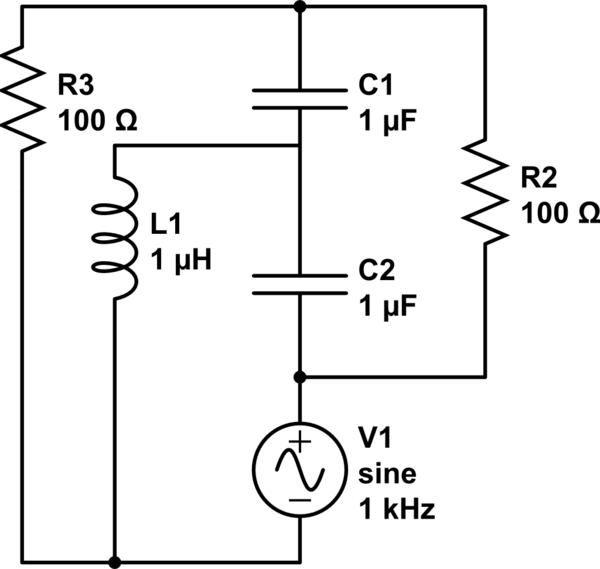
\includegraphics[width = 3.2in]{circ1.png}
\caption{Simple circuit with RLC-elements.}
\label{fig:circ1}
\end{figure}

An experienced electrical engineer can roughly estimate the behaviour of a circuit. As seen in Figure \ref{fig:circ1} and Figure \ref{fig:circ2}, electrical circuits often become more complicated and can easily confuse a less experienced engineer. Furthermore, it becomes hard to give a good estimate on the behaviour of such a circuit.
A program that confidently identifies the components of a schematic with their respective connections and translates those into a user-friendly SIMULINK model can substantially accelerate the understanding of given circuit. Analysing, modifying and storing a schematic becomes easy once it is properly digitized.

\begin{figure}[!ht]
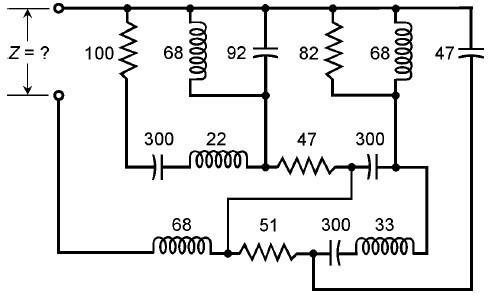
\includegraphics[width = 3.2in]{circ2.png}
\caption{A more complex circuit.}
\label{fig:circ2}
\end{figure}

% ------------------------------------

\section{Basic Idea}
\label{sec:basic}

The idea of this project is to analyse an image of an electrical schematic and scan it for components that form the circuit. By implementing algorithms that detect different components like resistors, capacitors, inductors and sources the schematic can be represented in SIMULINK. Furthermore, the connections between the components must be detected to fully describe the given circuit. Once the whole circuit is fed into the SIMULINK environment, analysis and modifications can be made.\\

For further implementation, by using already existing Optical Character Recognition (OCR) algorithms, the values of components like capacitors, resistors etc. can be identified to calculate more exact values (implementation of text recognition is not part of the project). This in turn enables the display of additional circuit information and their embedding in the model.

% ------------------------------------

\section{Method}

In a program solving the tasks defined in section \ref{sec:basic}, initially, an image of the schematic needs to be loaded and the region in which to look for the circuit needs to be specified. This way, it is possible to determine which components are part of the circuit.\\

%TODO Accurately identifying, classifying and analysing filters in an arbitrary schematic involves a lot of background knowledge about the design and structure of general electrical circuit schematics, perhaps by using external knowledge databases. In order to bypass the need for extensive databases and/or the conduction of network analyses, the image region in which to look for the filter is assumend to be known beforehand. While correctly identifying various types of filters in any given kind of electrical circuit sure needs experience in electrical engineering, identifying the general region in which filters could be found is a task that can also be accomplished by lesser experienced electrical engineers.\\
%Hab dafür keinen guten Ersatz gefunden

Besides the specifications of the components used in the circuit, aspects like material characteristics or production-related deviations from the desired state render a theoratically accurate description of the components' behavior very complex. In order to simplify the specification of the components and facilitate further usage of the retrieved circuit informations, we assume that our components are made out of ideal components, disregarding factors such as leakage current or non-linear behaviour.\\

Unfortunately, even in professional backgrounds, there exist several notations for electrical circuit components, complicating the analysis and usage of circuit schematics. Therefore, in the context of this work, we choose to abide by the standard defined by the American National Standard for \textit{Graphic Symbols for Electrical and Electronics Diagrams } (see \cite{standard1975graphic}) and, optionally, by the standard defined by the International Electrotechnical Commission (IEC).\\

\begin{figure}[!ht]
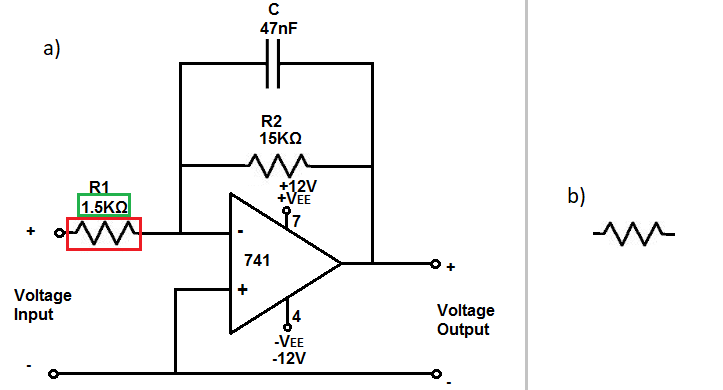
\includegraphics[width = 3.2in]{SchemeAndResistor.png}
\caption{a): Retrieved resistor and its specifications in a circuit schematic. b): Example template of a resistor to be used for solving the alignment problem.}
\label{fig:alignment}
\end{figure}

Identifying the different electrical components within a section of an image, in a generalized way, means solving alignment problems with pre-defined templates for every supported component. This means recognizing certain image features unique to a given component, such as the zig-zag shape of a resistor (see Figures \ref{fig:alignment} and \ref{fig:progression}, red box), in the image region. Moreover, using existing OCR modules, specifications of particular components can be retrieved aswell (in this example, there are no values given).\\

\begin{figure}[H]
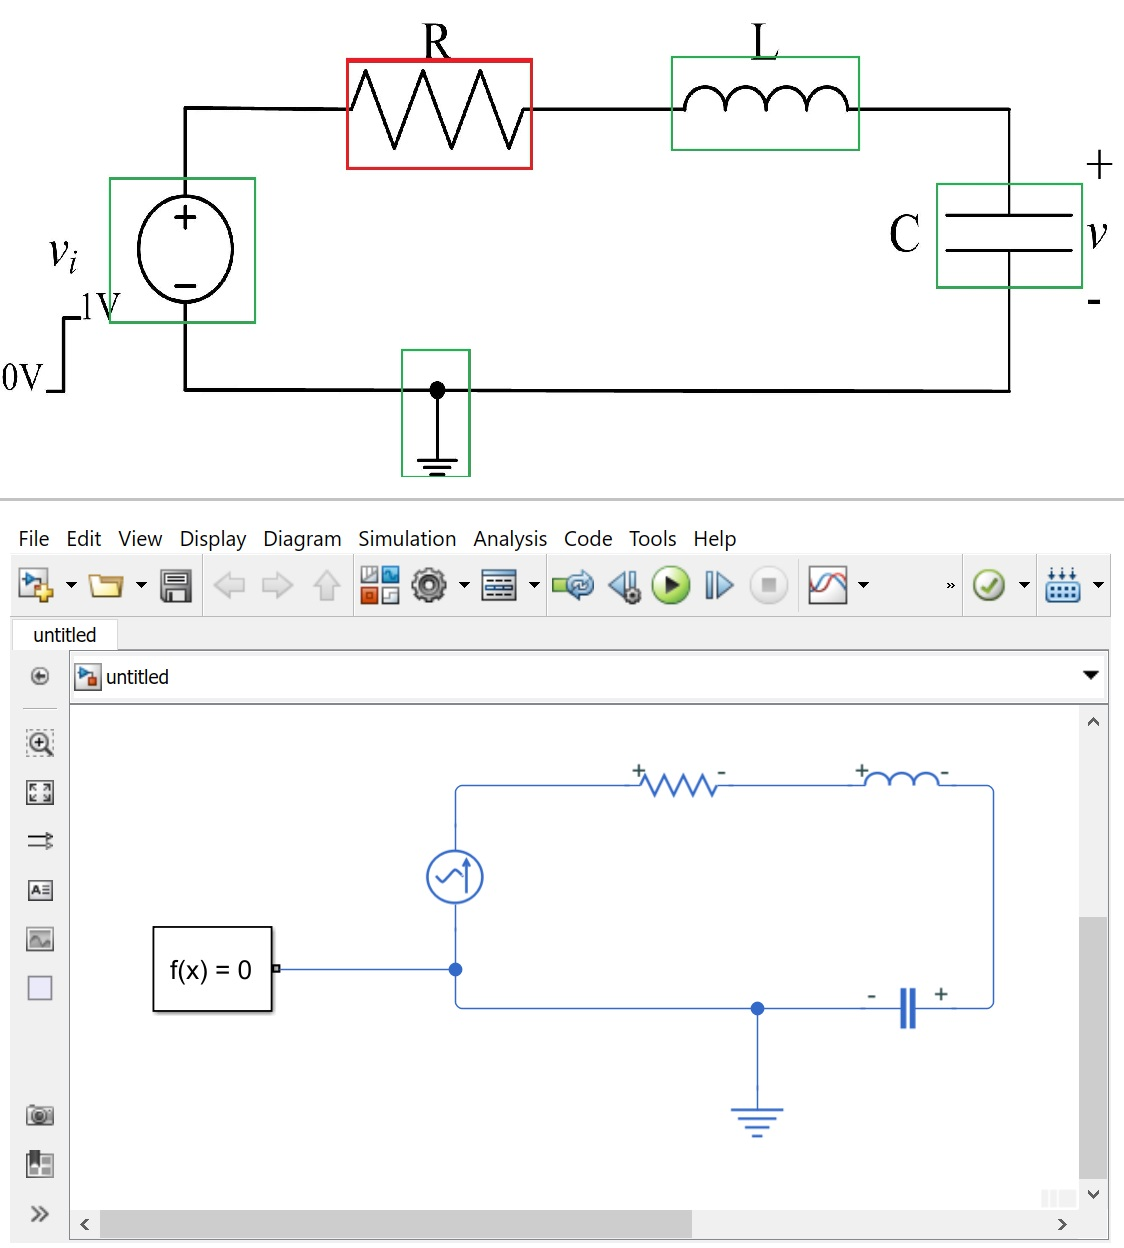
\includegraphics[width = 3.2in]{circ_progression.jpg}
\caption{Top: Circuit schematic and recognized circuit elements. Bottom: Resulting Circuit model in the SIMULINK environment.}
\label{fig:progression}
\end{figure}

After recognizing all components relevant to the circuit and component specifications made by numbers or text in the image, a SIMULINK model can be built within MATLAB (see Figure \ref{fig:progression}), containing the resulting electrical circuit and its characteristics (the circuit symbols used within MATLAB and SIMULINK abide to the American National Standard or the standard set by the IEC). The user can now start to analyze, modify or store the circuit using MATLAB and SIMULINK.

% ------------------------------------

\section{Experiment Data Sets}

Data sets for experiments, in this work, consist of images of electrical circuit diagrams. In practical circumstances, the visual representation of the circuit's  components can be distorted because the potentially hand-drawn diagram is captured with a camera - this means, the resulting image depends on factors such as illumination of the scene and the angle of the camera.

The electrical circuits used to test the system can either be obtained by using open sources of the internet or simply by designing our own simple schematics. In a first step, non-hand-drawn diagrams in the form of digital images would be analyzed in order to establish the basic functionality and structure of the recognition system. Thereafter, schematics would be printed out and subsequently scanned to simulate the engineer receiving a new electrical circuit diagram in paper form. Optionally - provided that the analysis of electrical circuits given in paper form is satisfactory - we will extend the functionality of this system to be able to analyse hand-drawn diagrams in addition to machine-drawn ones.

% ------------------------------------

\section{Related Work}

Basic object recognition in non-hand-drawn schematics, including the recognition of electrical circuit symbols, has been extensively covered for a long time in scientific literature as well as university lectures. Works like \cite{chhabra1997graphic} and \cite{llados2001symbol} give general overviews of object recognition methods whereas \cite{groen1985symbol} covers a possibility of specifically retrieving symbols in electrical diagrams. Object recognition based on hand-written or similarly distorted artifacts, on the other hand, is a problem with more relevancy in the present. Here, publications like \cite{ouyang2009visual} and \cite{feng2009line} are examples for solving the recognition task when dealing with hand-drawn diagrams.

{\small
\bibliographystyle{ieee}
\bibliography{egbib}
%}

\end{document}
